\documentclass[12pt]{article}
\usepackage[margin=1in]{geometry}
\usepackage{titling}
\usepackage[T1]{fontenc}
\usepackage{tabularx}
\usepackage{amsfonts}
\usepackage{graphicx}

\pretitle{\begin{center}\Huge\bfseries}
\posttitle{\par\end{center}\vskip 0.5em}
\preauthor{\begin{center}\Large}
\postauthor{\end{center}}
\predate{\par\large\centering}
\postdate{\par}

\title{Obliczenia naukowe - lab1}
\author{Jakub Musiał 268442}
\date{Październik 2023}

\begin{document}

\maketitle

\hspace{1cm}

\section*{Zadanie 1.1 -  Epsilon Maszunowy}
    \subsection*{Problem}
    Napisać program w języku \texttt{Julia} wyznaczający iteracyjnie wartości
    $\epsilon_{mach}$ takich, że: \newline
    \begin{equation}
        \left
        \lbrace
        \begin{array}{l}
            \epsilon_{mach} > 0 \\
            fl(1.0 + \epsilon_{mach}) > 1.0 \\
            fl(1.0 + \epsilon_{mach}) = 1 + \epsilon_{mach}
        \end{array}
        \right.
    \end{equation}
    \newline
    dla wszystkich typów zmiennopozycyjnych: \texttt{Float16}, \texttt{Float32}, \texttt{Float64}.
    \newline
    Można zauważyć, że $\epsilon_{mach}$ jest odległością od $1$ najmniejszej w zadanej arytmetyce liczby,
    której dodanie do $1$ skutkuje zmianą przechowywanej wartości.
    \newline

    \subsection*{Rozwiązanie}
        Liczbę maszynową $\epsilon_{mach}$ można otrzymać poprzez iteracyjne sprawdzanie kolejnych
        (co raz mniejszych) potęg liczby $2$, zaczynając od $2^0 = 1$,
        dopóki ograniczenia $(1)$ na wartość liczby $\epsilon_{mach}$ są spełnione.
        \newline\newline
        Programy z rozwiązaniem:
        \begin{itemize}
            \item \texttt{ex1/mach\_eps.jl}
            \item \texttt{ex1/mach\_eps.c}
        \end{itemize}

    \newpage

    \subsection*{Wyniki i obserwacje}
        Na podstawie \textit{tabeli 1} możemy zauważyć, że wyniki otrzymane iteracyjnie pokrywają się z tymi zwróconymi przez funkcję \texttt{eps},
        jak i z tymi zdefiniowanymi w standardzie języka \texttt{C}
        (wyłącznie w precyzji pojedynczej i podwójnej, jako że w języku \texttt{C} nie ma odpowiednika \texttt{Float16}).

        \begin{table}[h!]
            \centering
            \begin{tabularx}{0.9\textwidth}{c l l l}
                \hline
                Precyzja & Obliczone $\epsilon_{mach}$ & \texttt{eps} & \texttt{float.h} \\
                \hline
                Float16 & $0.000977$ & 0.000977 & brak \\
                Float32 & $1.1920929e-7$ & $1.1920929e-7$ & $1.192093e-07$ \\
                Float64 & $2.220446049250313e-16$ & $2.220446049250313e-16$ & $2.220446e-16$ \\
                \hline
            \end{tabularx}
            \caption{Wartości liczby $\epsilon_{mach}$ dla poszczególnych precyzji.}
            \label{table:macheps}
        \end{table}
        \noindent \newline\newline
        \textbf{Związek liczby $\epsilon_{mach}$ z precyzją arytmetyki:}
        \newline
        Precyzja arytmetyki $\epsilon$ jest określona wzorem:
        \begin{center}
        \begin{math}
            \epsilon = \frac{1}{2}\beta^{1 - t}
        \end{math}
        \end{center}
        Przy czym $\beta$ jest podstawą systemu, a $t$ jest liczbą cyfr mantysy. Wiedząc, że $\beta = 2$, możemy przekształcić powyższy wzór:
        \begin{center}
        \begin{math}
            \epsilon = \frac{1}{2} \cdot 2^{1 - t} = 2^{-t}
        \end{math}
        \end{center}
        Możemy zatem wyznaczyć wartości precyzji arytmetyk zmiennopozycyjnych.

        \begin{table}[h!]
            \centering
            \begin{tabularx}{0.78\textwidth}{c l l l}
                \hline
                Precyzja & $t$ & $\epsilon = fl(2^{-t})$ & $epsilon_{mach}$ \\
                \hline
                Float16 & $10$ & $0.000977$ & $0.000977$ \\
                Float32 & $23$ & $1.1920929e-7$ & $1.1920929e-7$ \\
                Float64 & $52$ & $2.220446049250313e-16$ & $2.220446049250313e-16$ \\
                \hline
            \end{tabularx}
            \caption{Porównanie wartości $\epsilon_{mach}$ oraz precyzji arytmetyki}
            \label{table:eps_macheps}
        \end{table}

        \noindent Na podstawie powyższej tabeli możemy stwierdzić, że $\epsilon = \epsilon_{mach}$.

\newpage

\section*{Zadanie 1.2 - Maszynowe eta}
    \subsection*{Problem}
    Napisać program w języku \texttt{Julia} wyznaczający iteracyjnie wartości
    $\eta_{mach} > 0$ dla wszystkich typów zmiennopozycyjnych: \texttt{Float16}, \texttt{Float32}, \texttt{Float64}.
    \newline
    Można zauważyć, że $\eta_{mach}$ jest najmniejszą nieujemną liczbą,
    którą da się zapisać w zadanej precyzji (nie wpada w przedział zera maszynowego).
    \newline

    \subsection*{Rozwiązanie}
        Liczbę maszynową $\eta_{mach}$ można otrzymać poprzez iteracyjne sprawdzanie kolejnych
        (co raz mniejszych) potęg liczby $2$, zaczynając od $2^0 = 1$,
        dopóki wyliczona wartość $\eta_{mach} > 0$.
        \newline\newline
        Program z rozwiązaniem: \texttt{ex1/mach\_eta.jl}

    \subsection*{Wyniki i obserwacje}
        Na podstawie \textit{tabeli 3} możemy zauważyć, że wyniki otrzymane iteracyjnie pokrywają się
        z tymi zwróconymi przez funkcję wbudowaną \texttt{nextfloat(0.0)}

        \begin{table}[h!]
            \centering
            \begin{tabularx}{0.52\textwidth}{c l l}
                \hline
                Precyzja & Obliczone $\eta_{mach}$ & \texttt{nextfloat(0.0)} \\
                \hline
                Float16 & $6.0e-8$ & $6.0e-8$ \\
                Float32 & $1.0e-45$ & $1.0e-45$ \\
                Float64 & $5.0e-324$ & $5.0e-324$ \\
                \hline
            \end{tabularx}
            \caption{Wartości liczby $\eta_{mach}$ dla poszczególnych precyzji.}
            \label{table:macheta}
        \end{table}

        \noindent Zauważmy, że liczba $\eta_{mach}$ w zapisie bitowym ma następującą postać:
        \begin{center}
        \begin{math}
            \eta_{mach}(precyzja) : 0 \;\; \underbrace{0...0}_{cecha} \;\;\; \underbrace{0...01}_{mantysa}
        \end{math}
        \end{center}
        Jest to zatem liczba nieznormalizowana, ponieważ cecha liczby $\eta_{mach}$ to same zera
        \newline\newline\newline
        \noindent\textbf{Związek liczby $\eta_{mach}$ z wartościa $MIN_{sub}$:}
        \newline
        Wiemy, że $MIN_{sub}$ jest namniejsza liczbą nieznormalizowaną w zadanej arytmetyce i jest określona wzorem:
        \begin{center}
        \begin{math}
            MIN_{sub} = 2^{1 - t} \cdot 2^{c_{min}} = 2^{1 - t + c_{min}}
        \end{math}
        \end{center}
        Zatem, wiedząc, że $c_{min} = -2^{d-1} + 2$ gdzie $d \equiv$ liczba bitów przeznaczonych na zapis cechy w standardzie \texttt{IEEE 754},
        możemy wyznaczyć wartości minimalne w postaci nieznormalizowanej dla zadanych precyzji.

        \newpage

        \begin{table}[h!]
            \centering
            \begin{tabularx}{0.73\textwidth}{c l l l l l}
                \hline
                Precyzja & $t$ & $d$ & $c_{min}$ & $MIN_{sub}$ & $\eta_{mach}$ \\
                \hline
                Float16 & $10$ & $5$ & $-14$ & $fl(2^{-24}) = 6.0e-8$ & $6.0e-8$ \\
                Float32 & $23$ & $8$ & $-126$ & $fl(2^{-149}) = 1.0e-45$ & $1.0e-45$ \\
                Float64 & $52$ & $11$ & $-1022$ & $fl(2^{-1074}) = 5.0e-324$ & $5.0e-324$ \\
                \hline
            \end{tabularx}
            \caption{Porównanie wartości $MIN_{sub}$ oraz $\eta_{mach}$}
            \label{table:minsub_macheta}
        \end{table}

        \noindent Na podstawie powyższej tabeli możemy stwierdzić, że $MIN_{sub} = \eta_{mach}$.
        \newline\newline\newline
        \noindent\textbf{Związek wartości $MIN_{nor}$ z funkcją \texttt{floatmin()}:}
        Wiemy, że wartość $MIN_{nor}$ możemy uzyscać ze wzoru:
        \begin{center}
        \begin{math}
            MIN_{nor} = 2^{c_{min}}
        \end{math}
        \end{center}
        Jak powyżej obliczamy $c_{min} = -2^{d-1} + 2$.
        \newline
        Zatem porównajmy zadany wzór z wartościami zwracanymi przez funkcję \texttt{floatmin()}.
        \begin{table}[h!]
            \centering
            \begin{tabularx}{0.91\textwidth}{c l l l l l}
                \hline
                Precyzja & $d$ & $c_{min}$ & $MIN_{nor}$ & \texttt{floatmin} \\
                \hline
                Float16 & $5$ & $-14$ & $6.104e-5$ & $6.104e-5$ \\
                Float32 & $8$ & $-126$ & $1.1754944e-38$ & $1.1754944e-38$ \\
                Float64 & $11$ & $-1074$ & $2.2250738585072014e-308$ & $2.2250738585072014e-308$ \\
                \hline
            \end{tabularx}
            \caption{Porównanie wartości $MIN_{nor}$ oraz funkcji \texttt{floatmin()}}
            \label{table:minnor_floatmin}
        \end{table}
        \noindent Z powyższej tabeli wynika, że funkcja wbudowana \texttt{floatmin()} języka \texttt{Julia}
        zwraca wartości $MIN_{nor}$ dla zadanej precyzji.

\newpage

\section*{Zadanie 1.3 - Maximum float}
    \subsection*{Problem}
    Napisać program w języku \texttt{Julia} wyznaczający iteracyjnie wartości
    $fl_{max}$ - największej liczby, którą da się zapisać w arytmetyce zmiennopozycyjnej -
    dla wszystkich typów zmiennopozycyjnych: \texttt{Float16}, \texttt{Float32}, \texttt{Float64}.

    \subsection*{Rozwiązanie}
        Liczbę $fl_{max}$ można otrzymać poprzez iteracyjne sprawdzanie kolejnych
        (co raz większych) potęg liczby $2$, zaczynając od $2^0 = 1$, dopóki wyliczona wartość $fl_{max} < \infty$,
        a następnie dodając coraz mniejsze potęgi liczby $2$, zaczynając od $2^{i_{max} - 1}$,
        ponownie dopóki wyliczona wartość $fl_{max} < \infty$
        \newline\newline
        Programy z rozwiązaniem:
        \begin{itemize}
            \item \texttt{ex1/max\_float.jl}
            \item \texttt{ex1/max\_float.c}
        \end{itemize}

    \subsection*{Wyniki i obserwacje}
        Na podstawie \textit{tabeli 5} możemy zauważyć, że wyniki otrzymane iteracyjnie pokrywają się
        z tymi zwróconymi przez funkcję wbudowaną \texttt{nextfloat(0.0)},
        jak i z tymi zdefiniowanymi w standardzie języka \texttt{C} (podobnie jak w zadaniu 1.1
        wyłącznie w precyzji pojedynczej i podwójnej, jako że w języku \texttt{C} nie ma odpowiednika \texttt{Float16}).

        \begin{table}[h!]
            \centering
            \begin{tabularx}{0.9\textwidth}{c l l l}
                \hline
                Precyzja & Obliczone $fl_{max}$ & \texttt{floatmax} & \texttt{float.h} \\
                \hline
                Float16 & $6.55e4$ & $6.55e4$ & brak \\
                Float32 & $3.4028235e38$ & $3.4028235e38$ & $3.402823e+38$ \\
                Float64 & $1.7976931348623157e308$ & $1.7976931348623157e308$ & $1.797693e+308$ \\
                \hline
            \end{tabularx}
            \caption{Wartości liczby $fl_{max}$ dla poszczególnych precyzji.}
            \label{table:floatmax}
        \end{table}

        \noindent Zauważmy, że liczba $fl_{max}$ w zapisie bitowym ma następującą postać:
        \begin{center}
        \begin{math}
            fl_{max}(precyzja) : 0 \;\; \underbrace{1...10}_{cecha} \;\;\; \underbrace{1...1}_{mantysa}
        \end{math}
        \end{center}

\newpage

\section*{Zadanie 2 - Kahan machine epsilon}
    \subsection*{Problem}
        Sprawdzić poprawność wzoru Kahana na oblicznanie wartości $\epsilon_{mach}$ dla wszystkich typów zmiennopozycyjnych: \texttt{Float16}, \texttt{Float32}, \texttt{Float64}.

    \subsection*{Rozwiązanie}
        Wzór Kahana:
        \begin{center}
        \begin{math}
            \epsilon_{kahan} = 3 \cdot (\frac{4}{3} - 1) - 1
        \end{math}
        \end{center}

        \noindent
        Program z rozwiązaniem: \texttt{ex2.jl}
        \newline

    \subsection*{Wyniki i obserwacje}
        \begin{table}[h!]
            \centering
            \begin{tabularx}{0.74\textwidth}{c l l}
                \hline
                Precyzja & $\epsilon_{kahan}$ & $\epsilon_{mach}$ \\
                \hline
                Float16 & $-0.000977$ & $0.000977$ \\
                Float32 & $1.1920929e-7$ & $1.1920929e-7$ \\
                Float64 & $-2.220446049250313e-16$ & $2.220446049250313e-16$ \\
                \hline
            \end{tabularx}
            \caption{Wartości liczby $\epsilon_{kahan}$ dla poszczególnych precyzji.}
            \label{table:kahan_macheps}
        \end{table}

        \noindent
        Na podstawie wyników w \textit{tabeli 7} możemy zauważyć, że wartości otrzymywane z wzoru Kahana
        są równe wartościom $\epsilon_{mach}$ co do wartości bezwzględnej, zatem, aby poprawić ten wzór należałoby
        nałożyć moduł na zwrócony wynik:
        \begin{center}
        \begin{math}
            \epsilon_{correct\:kahan} = | 3 \cdot (\frac{4}{3} - 1) - 1 |
        \end{math}
        \end{center}

\newpage

\section*{Zadanie 3 - Rozmieszczenie liczb w arytmetyce \newline zmiennopozycyjnej w podwójnej precyzji}
    \subsection*{Problem}
        Sprawdzić w języku \texttt{Julia}, czy liczby są równomiernie rozmieszczone w arytmetyce \texttt{Float64}
        w przedziałach: $[\frac{1}{2}, 1]$, $[1, 2]$ oraz $[2, 4]$
        \newline

    \subsection*{Rozwiązanie}
        Sprawdzenie wartości $x = 1 + k \cdot \delta$ dla $k \: \epsilon \: \{1, 2, ..., 2^{52}-1\}$
        \newline\newline
        Program z rozwiązaniem: \texttt{ex3.jl}
        \newline

    \subsection*{Wyniki i obserwacje}
        \subsubsection*{Przedział $[1, 2]$}
            Dla zadanej wartości $\delta = 2^{-52}$ uzyskujemy poniższe wartości:

            \begin{table}[h!]
                \centering
                \begin{tabularx}{0.74\textwidth}{c c}
                    \hline
                    Wartość & Postać binarna (znak bitu, cecha, mantysa) \\
                    \hline
                    $1.0000000000000002$ & $0\;\;01...1\;\;0...001$ \\
                    $1.0000000000000004$ & $0\;\;01...1\;\;0...010$ \\
                    $1.0000000000000007$ & $0\;\;01...1\;\;0...011$ \\
                    \vdots & \vdots \\
                    $1.9999999999999993$ & $0\;\;01...1\;\;1...101$ \\
                    $1.9999999999999996$ & $0\;\;01...1\;\;1...110$ \\
                    $1.9999999999999998$ & $0\;\;01...1\;\;1...111$ \\
                    \hline
                \end{tabularx}
                \caption{Rozkład liczb podwójnej precyzji w przedziale $[1, 2]$}
                \label{table:arrangement_in_1_2}
            \end{table}

            \noindent W \textit{tabeli 8} możemy zauważyć, że dodanie $\delta = 2^{-52}$ do liczby $x$ z przedziału $[1, 2]$
            powoduje dodanie wartości binarnej $1$ do $m_x$ (mantysy liczby $x$). Zatem możemy stwierdzić, że
            liczby w tym przedziale są równomiernie rozmieszczone z krokiem $2^{-52}$.
            \newline

        \subsubsection*{Przedział $[\frac{1}{2}, 1]$}
            Wiemy, że liczb w przedziale $[\frac{1}{2}, 1]$ jest tyle samo, co w przedziale $[1, 2]$, ponieważ
            liczby w zadanym przedziale $[2^i, 2^{i + 1}]$ mają tę samą cechę, a możliwych wartości mantysy
            jest ${2^t = 2^{52}}$. Zauważmy także, że dla $i = j - 1$ ($i, j \equiv $ wartości cechy) liczby reprezentowane
            przez tę samą mantysę z cechą $i$ są dwukrotnie mniejsze od tych z cechą $j$, czyli $x_i = 2^{-1} \cdot x_j$. \newline
            Stąd możemy założyć, że dla przedziału $[\frac{1}{2}, 1]$ powinniśmy przyjąć krok $\delta = 2^{-52 - 1} = 2^{-53}$

            \begin{table}[h!]
                \centering
                \begin{tabularx}{0.74\textwidth}{c c}
                    \hline
                    Wartość & Postać binarna (znak bitu, cecha, mantysa) \\
                    \hline
                    $0.5000000000000001$ & $0\;\;01...10\;\;0...001$ \\
                    $0.5000000000000002$ & $0\;\;01...10\;\;0...010$ \\
                    $0.5000000000000003$ & $0\;\;01...10\;\;0...011$ \\
                    \vdots & \vdots \\
                    $0.9999999999999997$ & $0\;\;01...10\;\;1...101$ \\
                    $0.9999999999999998$ & $0\;\;01...10\;\;1...110$ \\
                    $0.9999999999999999$ & $0\;\;01...10\;\;1...111$ \\
                    \hline
                \end{tabularx}
                \caption{Rozkład liczb podwójnej precyzji w przedziale $[\frac{1}{2}, 1]$}
                \label{table:arrangement_in_05_1}
            \end{table}

            \noindent Na podstawie uzyskanych wyników powtórzonego eksperymentu dla przedziału $[\frac{1}{2}, 1]$,
            możemy stwierdzić, że nasze założenie było poprawne, a liczby w zadanym przedziale są rozmieszczone równolegle
            z krokiem $\delta = 2^{-53}$.
            \newline

        \subsubsection*{Przedział $[2, 4]$}
            Przeprowadziwszy rozumowanie analogiczne do tego dla przedziału $[\frac{1}{2}, 1]$, możemy przyjąć,
            że dla przedziału $[2, 4]$ powinniśmy sprawdzić rozmieszczenie liczb z krokiem $\delta = 2^{-51}$.

            \begin{table}[h!]
                \centering
                \begin{tabularx}{0.74\textwidth}{c c}
                    \hline
                    Wartość & Postać binarna (znak bitu, cecha, mantysa) \\
                    \hline
                    $2.0000000000000004$ & $0\;\;10...0\;\;0...001$ \\
                    $2.000000000000001$  & $0\;\;10...0\;\;0...010$ \\
                    $2.0000000000000013$ & $0\;\;10...0\;\;0...011$ \\
                    \vdots & \vdots \\
                    $3.9999999999999996$ & $0\;\;10...0\;\;1...101$ \\
                    $3.999999999999999$  & $0\;\;10...0\;\;1...110$ \\
                    $3.9999999999999987$ & $0\;\;10...0\;\;1...111$ \\
                    \hline
                \end{tabularx}
                \caption{Rozkład liczb podwójnej precyzji w przedziale $[2, 4]$}
                \label{table:arrangement_in_2_4}
            \end{table}

            \noindent Tutaj również możemy zauważyć, że liczby z zadanego przedziału są równolegle rozmieszczone
            dla założonej $\delta$, która jest tutaj równa $2^{-51}$.
            \newline

        \subsubsection*{Ogólne spostrzerzenie}
            Możemy zauważyć, że w arytmetyce zmiennopozycyjnej liczby w przedziałach $[2^i, 2^{i + 1}]$
            są równomiernie rozmieszczone z krokiem $\delta = 2^{-t + i}$, gdzie $t \equiv$ liczba bitów mantysy.
            \newline
            Z tego wynika fakt, że liczby w przedziałach $[2^i, 2^{i + 1}]$ oraz $[2^j, 2^{j + 1}]$ mają inne rozmieszczenie
            dla $i \ne j$. Dokładniej - im wieksza jest wartość $i$, tym "rzadziej" rozmieszczone są
            liczby w przedziale $[2^i, 2^{i + 1}]$.

\newpage

\section*{Zadanie 4 - Liczby odwrotne}
    \subsection*{Problem}
        a. Znaleźć w języku \texttt{Julia} liczbę zmiennopozycyjną $x$ w precyzji \texttt{Float64} taką, że: \newline
        \begin{equation}
            \left
            \lbrace
            \begin{array}{l}
                x \epsilon (1, 2) \\
                x \cdot \frac{1}{x} \ne 1 \iff fl(x \cdot fl(\frac{1}{x})) \ne 1
            \end{array}
            \right.
        \end{equation}

        \noindent b. Znaleźć najmniejszą liczbę $x$ spełniającą $(2)$

    \subsection*{Rozwiązanie}
        Zaczynając od $x =$ \texttt{nextfloat(1)} (ponieważ $x > 1$) sprawdzać kolejne liczby zmiennoprzecinkowe
        (przypisując $x \leftarrow$ \texttt{nextfloat(x)}), dopóki $x < 2 \land x \cdot \frac{1}{x} = 1$.
        \newline\newline
        Taki algorytm znajdzie najmniejszą liczbę $x$ spełniającą warunki $(2)$.
        \newline\newline
        Program z rozwiązaniem: \texttt{ex4.jl}
        \newline

    \subsection*{Wyniki i obserwacje}
        Najmniejszą liczbą spełniającą warunki zadania jest $x = 1.000000057228997$.
        \newline\newline
        Możemy zauważyć, że dokładność obliczeń (precyzja arytmetyki) ma znaczący wpływ na uzyskiwane wyniki,
        dlatego należy mieć to na uwadze, implementująć algorytmy, by uniknąć lub zminimalizować wystąpienia
        takich błędów i ich kumulowania się

\newpage

\section*{Zadanie 5 - Iloczyn skalarny}
    \subsection*{Problem}
        Zaimplementować w języku \texttt{Julia} algorytm obliczania iloczynu skalarnego dwóch wektorów,
        sumując przemnożone elementy na cztery sposoby: w przód, w tył, od największego do najmniejszego oraz od najmniejszego do najwięszego
        \noindent Algorytmy należy przetestować dla precyzji \texttt{Float32} oraz \texttt{Float32}.
        \newline

    \subsection*{Rozwiązanie}
        Program z rozwiązaniem: \texttt{ex5.jl}
        \newline

    \subsection*{Wyniki i obserwacje}
        Znając rzeczywistą wartość iloczynu skalarnego zadanych wektorów $x$ oraz $y$:
        \begin{center}
        \begin{math}
            S_{true} = 1.0065710699999998e-11
        \end{math}
        \end{center}
        Możemy obliczyć błąd względny uzyskanych wyników wg wzoru: $\delta = \frac{|S - S_{true}|}{S_{true}}$
        \newline

        \begin{table}[h!]
            \centering
            \begin{tabularx}{0.67\textwidth}{l l l}
                \hline
                Algorytm & $S$ & $\delta$ \\
                \hline
                W przód & $-0.4999443$ & $4.966805766328285e10$ \\
                W tył & $-0.4543457$ & $4.5137965582009605e10$ \\
                Od najwięszych & $-0.5$ & $4.967359135506108e10$ \\
                Od najmniejszych & $-0.5$ & $4.967359135506108e10$ \\
                \hline
            \end{tabularx}
            \caption{Wartości iloczynu skalarnego wraz z błędem względnym w precyzji \texttt{Float32}}
            \label{table:dot_prod_32}
        \end{table}

        \begin{table}[h!]
            \centering
            \begin{tabularx}{0.78\textwidth}{l l l}
                \hline
                Algorytm & $S$ & $\delta$ \\
                \hline
                W przód & $1.0251881368296672e-10$ & $9.184955313981629$ \\
                W tył & $-1.5643308870494366e-10$ & $16.54118664516592$ \\
                Od najwięszych & $0.0$ & $1.0$ \\
                Od najmniejszych & $0.0$ & $1.0$ \\
                \hline
            \end{tabularx}
            \caption{Wartości iloczynu skalarnego wraz z błędem względnym w precyzji \texttt{Float64}}
            \label{table:dot_prod_64}
        \end{table}

        \noindent Na podsawie wyników z \textit{tabeli 12} możemy stwerdzić, że kolejność sumowania elementów w arytmetyce
        zmiennopozycyjnej może mieć duże znaczenie dla otrzymanego wyniku.
        \newline
        Dodatkowo zauważmy, że wektory $x$ oraz $y$ są do siebie prawie prostopadłe - ich iloczyn skalarny jest bliski $0$.
        Zatem biorąc pod uwagę fakt, że otrzymane błędy sięgały nawet $\sim1600\%$, możemy stwirdzić,
        że oblicznia bliskie $0$ mogą generować duże błędy.

\newpage

\section*{Zadanie 6 - Równoważne wunkcje}
    \subsection*{Problem}
        Wyznaczyć wartości zadanych funkcji:
        \begin{itemize}
            \item $f(x) = \sqrt{x^2 + 1} - 1$
            \item $g(x) = x^2 / (\sqrt{x^2 + 1} + 1)$
        \end{itemize}
        W arytmetyce zmiennopozycyjnej w podwójnej precyzji dla $x = 8^i : i \: \epsilon \: \mathbb{N}^+$
        \newline

    \subsection*{Rozwiązanie}
        Program z rozwiązaniem: \texttt{ex6.jl}

    \subsection*{Wyniki i obserwacje}
        Eksperyment przeprowadziłem dla $i \: \epsilon \: \{1, 2, ..., 16\}$.

        \begin{table}[h!]
            \centering
            \begin{tabularx}{0.78\textwidth}{c l l}
                \hline
                Exponent: $i$ & $f(x)$ & $g(x)$ \\
                \hline
                $1$ & $0.0077822185373186414$ & $0.0077822185373187065$ \\
                $2$ & $0.00012206286282867573$ & $0.00012206286282875901$ \\
                $3$ & $1.9073468138230965e-6$ & $1.907346813826566e-6$ \\
                $4$ & $2.9802321943606103e-8$ & $2.9802321943606116e-8$ \\
                $5$ & $4.656612873077393e-10$ & $4.6566128719931904e-10$ \\
                $6$ & $7.275957614183426e-12$ & $7.275957614156956e-12$ \\
                $7$ & $1.1368683772161603e-13$ & $1.1368683772160957e-13$ \\
                $8$ & $1.7763568394002505e-15$ & $1.7763568394002489e-15$ \\
                $9$ & $0.0$ & $2.7755575615628914e-17$ \\
                $10$ & $0.0$ & $4.336808689942018e-19$ \\
                $11$ & $0.0$ & $6.776263578034403e-21$ \\
                $12$ & $0.0$ & $1.0587911840678754e-22$ \\
                $13$ & $0.0$ & $1.6543612251060553e-24$ \\
                $14$ & $0.0$ & $2.5849394142282115e-26$ \\
                $15$ & $0.0$ & $4.0389678347315804e-28$ \\
                $16$ & $0.0$ & $6.310887241768095e-30$ \\
                \hline
            \end{tabularx}
            \caption{Wartości równoważnych funkcji $f$ oraz $g$}
            \label{table:equiv_func}
        \end{table}

        \noindent Na podstawie powyższej tabeli możemy stwierdzić, że mimo matematycznej równoważności
        funkcji $f$ i $g$, nie są one równoznaczne w arytmetyce zmiennopozycyjnej.
        \newline
        W tym przypadku bardziej wiarygodne wyniki zwraca funkcja $g$.
        Niedokładność funkcji $f$ może wynikać z tego, że wykonuje ona operację odejmowania bliskich siebie wartości.


\newpage

\section*{Zadanie 7 - Przybliżenie pochodnej}
    \subsection*{Problem}
        Wyznaczyć w języku \texttt{Julia} przybliżone wartości pochodnej funkcji $f(x) = \sin{x} + \cos{3x}$, korzystając z wzoru:
        \begin{center}
        \begin{math}
            f'(x_0) \approx \tilde{f'}(x) = \frac{f(x_0 + h) - f(x_0)}{h}
        \end{math}
        \end{center}
        Dla $x_0 = 1 \land h = 2^{-n} : n \: \epsilon \: \{0, 1, ..., 54\}$
        \newline

    \subsection*{Rozwiązanie}
        Program z rozwiązaniem: \texttt{ex7.jl}
        \newline

    \subsection*{Wyniki i obserwacje}
        Wiedząc, że $f'(x0) = \cos(x_0) - 3 \cdot sin(3x_0)$ możemy porównać otrzymane przybliżenia
        pochodnej funkcji $f$ z jej rzeczywistą wartością oraz obliczyć błąd bezwzględny tych przybliżeń.

        \begin{figure}[h]
            \centering
            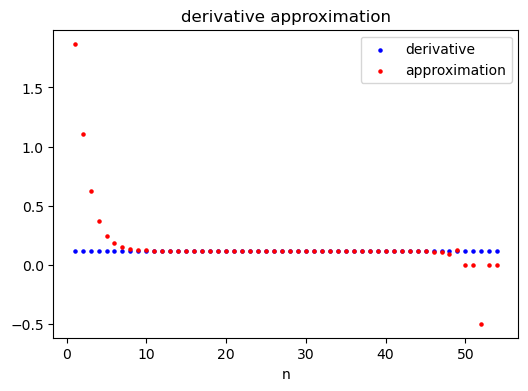
\includegraphics[width=0.8\linewidth]{ex7_deriv_approx.png}
            \caption{Przybliżenie pochodniej funkcji $f$}
            \label{fig:deriv_approx}
        \end{figure}

        \newpage
        \noindent
        Na podstawie \textit{wykresu 1} mozemy zauważyć, że na początku zmniejszanie wartości $h$
        powoduje bardzo szybki wzrost dokładności przybliżenia, jednak od pewnego momentu przybliżenie
        to przestaje być bardziej dokładne, a nawet zaczyna być coraz mniej, co wynika z tego, że $h \approx 0 \Rightarrow fl(1 + h) = 1$.
        \newline
        Można to zauważyć także na \textit{wykresie 2}, który bardzo dobrze pokazuje spadek dokładności
        przybliżenie pochodnej funkcji $f$ dla bardzo małych wartości $h$.
        \newline\newline\newline

        \begin{figure}[h]
            \centering
            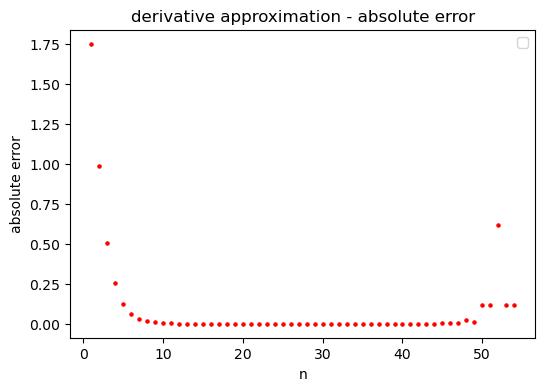
\includegraphics[width=0.8\linewidth]{ex7_deriv_error.png}
            \caption{Błąd bezwzględny przybliżenia pochodnej funkcji $f$}
            \label{fig:deriv_error}
        \end{figure}

\end{document}
